\documentclass[mathserif,serif]{beamer}

\usepackage{graphicx}
\shorthandoff{=}

%\setbeamertemplate{blocks}[rounded][shadow=true]
\setbeamertemplate{background canvas}[vertical shading][bottom=white,top=structure.fg!25]

\mode<presentation>

\newcommand {\framedgraphic}[2] {
    \begin{frame}{#1}
        \begin{center}
            \includegraphics[width=\textwidth,height=0.8\textheight,keepaspectratio]{#2}
        \end{center}
    \end{frame}
}


\title{SWOP iteratie 2}
\author{Pablo en Co (groep 2)}
\institute{KU Leuven}
\date{2015}

\begin{document}

  \frame{\titlepage}

  \begin{frame}{High Level}
    \begin{center}
        \includegraphics[width=\textwidth,height=0.8\textheight,keepaspectratio]{../../diagrams/high_level_uml.eps}
    \end{center}
  \end{frame}

  \begin{frame}{Task interpretatie}
      \begin{center}
      
\includegraphics[width=\textwidth,height=0.8\textheight,keepaspectratio]{../../diagrams/task_dfs.eps}
      \end{center}
  \end{frame}

  \begin{frame}{Status update}
      \begin{center}
      \includegraphics[width=\textwidth,height=0.9\textheight,keepaspectratio]{../../diagrams/sequence_update_task_status_simple_uml.eps}
      \end{center}
  \end{frame}

  \begin{frame}{Plan task}
      \begin{center}
      \includegraphics[width=\textwidth,height=0.9\textheight,keepaspectratio]{../../diagrams/sequence_planTask_simple_uml.eps}
      \end{center}
  \end{frame}
  
  \begin{frame}{Create Task}
      \begin{center}
      \includegraphics[width=\textwidth,height=0.6\textheight,keepaspectratio]{../../diagrams/sequence_createTask_simple_uml.eps}
        \begin{itemize}
        \item projectwrapper
        \item projectdata
        \item createtaskfor(projectwrapper, projectdata)
        \end{itemize}
      \end{center}
  \end{frame}

  \begin{frame}{Testing}
      \begin{center}
      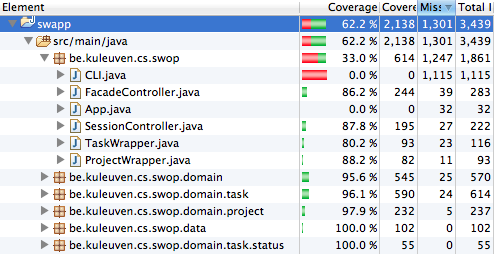
\includegraphics[width=\textwidth,height=0.6\textheight,keepaspectratio]{code_coverage.png}
        \begin{itemize}
        \item Unit tests per klasse
        \item Use case tests $\rightarrow$ Testing UI
        \item Scenario test
        \item Fuzz testing $\rightarrow$ Button masher UI
        \end{itemize}
      \end{center}
  \end{frame}

% etc
\end{document}




%%% Local Variables:
%%% mode: latex
%%% TeX-master: " RET"
%%% End:
